% =====================================================================
%  Paper-style synthesis of the simple-task work: the two source methods
%  (Yang et al.; Davidson et al.) as reproduced, the common design, every
%  head-selection rule compared at the same set sizes, and which ones work best.
%  Capped comparison: scripts/e13_report.py (paper/tables/e13_*, paper/figures/e13_*).
%  Earlier comparisons (App. C): scripts/synthesis_report.py (synth_*).
%  Compile with Tectonic (XeTeX): non-Latin words in the word lists need fontspec.
% =====================================================================
\documentclass[10pt,a4paper]{article}

\usepackage{fontspec}
\newfontfamily\cjkfont{FandolSong-Regular.otf}
\newfontfamily\jafont{ipaexm.ttf}
\newfontfamily\cyrfont{cmunrm.otf}
\newcommand{\zh}[1]{{\cjkfont #1}}
\newcommand{\ja}[1]{{\jafont #1}}
\newcommand{\ru}[1]{{\cyrfont #1}}
\usepackage[margin=2.2cm]{geometry}
\usepackage{amsmath,amssymb}
\usepackage{booktabs,tabularx,array}
\usepackage{xltabular}
\usepackage{graphicx}
\usepackage{float}
\usepackage{enumitem}
\usepackage{xcolor}
\usepackage{caption}
\usepackage[round,authoryear]{natbib}
\usepackage[colorlinks=true,linkcolor=blue!50!black,citecolor=green!40!black,urlcolor=blue!60!black]{hyperref}

\setlist{nosep,leftmargin=*}
\captionsetup{font=small,labelfont=bf}
\renewcommand{\arraystretch}{1.12}
\setlength{\emergencystretch}{3em}
\newcolumntype{L}{>{\raggedright\arraybackslash}X}

\title{Small Head Sets for Simple Tasks\\[2pt]
\large Lexical task heads, function-vector heads and attention filters in Llama-3.1-8B-Instruct}
\author{Filippo Merlo}
\date{11 November 2026}

\begin{document}
\maketitle

\begin{abstract}
We look for small sets of attention heads whose mean output, written into a prompt that does not state the task, makes Llama-3.1-8B-Instruct perform it, on 14 simple tasks. We re-implement two published ways of choosing heads, by the words a head decodes \citep{yang2026shared} and by its causal effect \citep{davidson2025different}, read heads with Head-JLens as well as with the logit lens, and add rules that combine what a head decodes with where it attends. All rules are then compared at the same set sizes, 20 to 80 heads, both as one set per task and as one set for all tasks, with heads chosen on half of each task's items and tested on the other half. Head-JLens finds more heads that carry the task than the logit lens, and the hand-written word lists are the weak point of the lexical method. Per task, heads that attend to the instruction's task words and little to the first token match or beat the causal ranking at every size, without any patching during selection. For one set shared by all tasks the causal ranking is best, once a few generic heads that decode the same tokens on every task are removed. Task types rest on different heads: translations on attention-filtered heads, morphology on causally ranked ones. Readings and attention are enough to find a small head set for each task; one set for all tasks still needs the causal score.
\end{abstract}

% =====================================================================
\section{Introduction}

A task representation in a language model can be located by finding the attention heads whose outputs, averaged over prompts that state the task and written into a prompt that does not, make the model perform the task \citep{todd2024function}. Two recent studies choose those heads in different ways. \citet{yang2026shared} decode each head's output at the last prompt token with the logit lens and call a head a \emph{lexical task head} when its top tokens contain words describing the task (\emph{opposite}, \emph{capital}). \citet{davidson2025different} rank heads by their causal effect on the answer when the prompt's instruction is replaced by uninformative text, and sum the mean outputs of the top heads into an \emph{instruction function vector}.

Our goal is the smallest set of heads that represents the tasks well, ideally one set for all of them. We reproduce both methods on the same model and tasks, add a second readout, Head-JLens \citep{merlo2026headjlens}, and build selection rules from what the reproductions show: word lists taken from what heads decode, and filters on where a head attends. We then compare all rules on equal terms. Every rule ranks the heads and gives its top 20, 40, 60 and 80, once per task and once for all tasks, with heads chosen on one half of each task's items and tested on the other.

The paper is organised linearly: the common setup (Sec.~\ref{sec:setup}), the two reproductions (Sec.~\ref{sec:repro}), the design of the comparison (Sec.~\ref{sec:approaches}), its results (Sec.~\ref{sec:results}), and the approaches we would keep (Sec.~\ref{sec:best}). The earlier comparisons at uneven set sizes, which led to this design, are in App.~\ref{app:earlier}. Only simple tasks are covered.

% =====================================================================
\section{Setup}\label{sec:setup}

\paragraph{Model and tasks.} Llama-3.1-8B-Instruct in bfloat16, the main model of \citet{yang2026shared} and the only one with released Head-JLens matrices. The 14 simple tasks shared by both source studies, with the datasets of \citet{todd2024function}: antonym, synonym, singular--plural, present--past, country--capital, country--currency, landmark--country, park--country, product--company, next-item, prev-item, English--French, English--German, English--Spanish. We group them as word relations, morphology, facts, sequences and translations. Prompts follow \citet{yang2026shared}: raw text without the chat template; five instruction templates per task (the cloze form ``The antonym of \{x\} is'' and four of the form ``\textless instruction\textgreater{} Q: \{x\}\textbackslash nA:''); example prompts with 1 to 30 shots (`` x$_1$: y$_1$; x:''); and the zero-shot prompt `` x:'', which states no task. Decoding is greedy.

\paragraph{Reading a head.} For head $h$ of layer $l$, $z_{l,h}$ is its output at the last prompt token before the output projection and $c_{l,h}=W_O^{(h)}z_{l,h}$ its write to the residual stream. With $q_v$ the unembedding row of token $v$ scaled by the final norm's gain, the two readouts score $v$ by
\[
\text{Logit-head: } q_v^\top c_{l,h}, \qquad \text{J-head: } q_v^\top J_{l,h}\, z_{l,h},
\]
where $J_{l,h}$ is the head's part of the Jacobian map of Head-JLens, fitted on WikiText-103 \citep{merlo2026headjlens}. J-head reads the head through the layers that follow it; Logit-head is the readout of \citet{yang2026shared}. A head \emph{decodes} a word on a prompt when one of the word's token forms is among its 10 highest-scoring tokens.

\paragraph{Testing a head set.} A set is tested by mean patching \citep[Sec.~2.3.2]{yang2026shared}. For each head in the set, its mean output over prompts that state the task (correctly answered, items not patched) is computed; at the last token of the patched prompt, the head's output is replaced by $\alpha$ times this mean, and the model generates its answer. There are two checks.
\begin{itemize}
\item \textbf{Check 1} patches the zero-shot prompts of items the model answers correctly with one shot. The prompt says nothing about the task, so unpatched accuracy is near zero, and a gain means the set brings the task in. This is the main test, and the only one in the capped comparison.
\item \textbf{Check 2} patches the 1-shot prompts of items the model answers \emph{wrongly} with one shot (unpatched accuracy 0). The prompt already shows the task and the answer format, so this check measures repair rather than transfer. It was run in the reproductions and the earlier comparisons, where it did not separate good sets from mediocre ones (App.~\ref{app:earlier}).
\end{itemize}
A \emph{control} patches the same heads with the mean of a related task (the pairing of \citealp{yang2026shared}, e.g.\ antonym with synonym); a set carries its task when its own mean helps and the control mean does not.

\paragraph{Scoring.} A reply is correct when it begins with the whole reference answer as words, ignoring case, accents, punctuation and a leading article. This replaces the first-token match of \citet{yang2026shared}, which marks any number correct on next- and prev-item and a capitalised German noun wrong. The same score selects the correctly answered prompts used everywhere else.

\paragraph{Held-out protocol.} In the comparison of selection rules (Secs.~\ref{sec:approaches} and~\ref{sec:results}), every quantity that depends on items is chosen on one half of each task's items and tested on the other. The items are shuffled once (seed 0) and split into halves $A$ and $B$; fold~1 chooses on $A$ and tests on $B$, fold~2 the reverse. ``Chosen'' covers the prompts whose heads are read, the word lists, the generic heads, the head rankings, the causal scores of Davidson et al., and the task and control means. The means are rule-style: one per instruction template, over its first 100 correctly answered prompts of the choosing half; each patched item is patched with each of the five means and accuracy is averaged over them. Up to 100 items per task and fold are patched (as few as 58 on next-item). The scaling is $\alpha\in\{1,2\}$. For each fold, $\alpha$ is the value that was better on the other fold for the same task and set (cross-fitting; ties go to $\alpha=1$), so it is never chosen on the items it is scored on. Random sets are scored at the $\alpha$ of the set they are matched to. Reported numbers are means of the two folds. Replies stop at a newline, the example delimiter or 16 tokens. Every run is single and greedy, and we report accuracies only, without intervals.

% =====================================================================
\section{Reproducing the two source methods}\label{sec:repro}

\subsection{\texorpdfstring{Lexical task heads \citep{yang2026shared}}{Lexical task heads (Yang et al., 2026)}}

\paragraph{Method.} A head is a lexical task head for a task and prompt style if, on at least 10\% of 100 correctly answered prompts, at least one of its top-10 Logit-head tokens is in a hand-written term list for the task (2 to 22 tokens). The prompts are those of the most accurate instruction template (rule style) or the 5-shot prompts (example style). The set is then tested by mean patching with each wording's own mean, at 15 values of $\alpha$ from $-10$ to $10$.

\paragraph{Fidelity.} We re-run their code's data, templates, term lists, control pairs and parameters (Table~\ref{tab:fid-yang}). We depart from it in four places, each by choice: the padding mask, the J-head readout, the answer score, and bfloat16 instead of float32, the precision in which the lens was fitted. Their code passes batches of 20 left-padded prompts without an attention mask, so the model attends to the padding; we mask it. Run in their code's own setting (padding attended, first-token score), our Logit-head counts are within one head of their Figs.~79 and~88 on every task (rule style: 250 heads over the 14 tasks against their 247; example style: 127 against 130).

\begin{table}[H]
\centering\small
\begin{tabularx}{\textwidth}{@{}>{\raggedright\arraybackslash}p{3.3cm}LL@{}}
\toprule
Setting & \citet{yang2026shared} & Here \\
\midrule
Model, precision & Llama-3.1-8B-Instruct, float32 & same model, bfloat16 \\
Tasks, templates, term lists & 14 Todd et al.\ tasks; first 5 of the 6 templates; their lists & same \\
Batching & 20 left-padded prompts, padding attended & same batches, padding masked \\
Readout & Logit-head & Logit-head and J-head \\
Head criterion & top 10, $\geq$1 term, $\geq$10\% of the first 100 correct prompts & same \\
Answer score & first generated token & generated reply, flexible score \\
Means, $\alpha$, control & one mean per wording; 15 values $-10$..$10$; their control map & same \\
Check 1 & zero-shot prompts (paper, App.~G.1); no released script & as the paper \\
Check 2 & 1-shot prompts answered wrongly (the released script) & same; control added in the held-out runs \\
\bottomrule
\end{tabularx}
\caption{Lexical task heads: their setting and ours.}
\label{tab:fid-yang}
\end{table}

\paragraph{What reproduces.} Logit-head finds lexical task heads for every task. In check~1, which their paper describes, patching gains only on the fact tasks (and a few more with example means) and does nothing on antonym, synonym, present--past, prev-item and the translations. The per-task curves of their App.~G.1 (Figs.~57 and~62), which the text attributes to zero-shot patching, reproduce only in check~2, the setting of their one released causal script. There every task gains, with the largest and smallest gains on the same tasks as in their figures. Their headline finding thus holds in check~2. In check~1, the lexical heads carry only some task types.

\paragraph{J-head against Logit-head} (Table~\ref{tab:readouts}). J-head finds 50 to 70\% more heads; most of the added ones lie in layers 10--19, where Logit-head finds few. The heads only J-head finds have causal effects of their own, and J-head sets are at least as effective as Logit-head sets in both checks and both styles. The lead is not a matter of set size: comparing the top 5, 10 and 20 heads of each readout, most of J-head's leads remain and none reverses, while none of Logit-head's few leads remains. J-head does not contain the Logit-head set (only on 4 of 28 task--style pairs). From here on all sets are read with J-head. The one later comparison of readouts, LLM-scored heads on two tasks, mostly points the same way.

\begin{table}[H]
\centering\small
% Generated by scripts/synthesis_report.py.
\begin{tabular}{@{}lccccccccc@{}}
\toprule
 & \multicolumn{3}{c}{Heads (sum over tasks)} & \multicolumn{3}{c}{Check 1 effect} & \multicolumn{3}{c}{Check 2 effect} \\
\cmidrule(lr){2-4}\cmidrule(lr){5-7}\cmidrule(lr){8-10}
Style & L & J & L$\cap$J & L & J & J only & L & J & J only \\
\midrule
Rule & 240 & 370 & 199 & 0.17 & 0.19 & 0.10 & 0.26 & 0.32 & 0.27 \\
Example & 141 & 237 & 107 & 0.22 & 0.32 & 0.24 & 0.33 & 0.43 & 0.38 \\
\bottomrule
\end{tabular}

\caption{Lexical task heads under both readouts (items not held out). Heads: summed over the 14 tasks. Effect: highest accuracy over the 15 values of $\alpha$, averaged over the style's five means, minus unpatched accuracy; mean over tasks. J only: heads J-head finds and Logit-head does not.}
\label{tab:readouts}
\end{table}

\subsection{\texorpdfstring{Instruction function vectors \citep{davidson2025different}}{Instruction function vectors (Davidson et al., 2025)}}

\paragraph{Method.} Each head is scored by its causal indirect effect: the gain in probability of the answer's first token when that head alone is set to its mean output, on prompts whose instruction is replaced by uninformative text of matched length and log-probability. There are three kinds of such text: token sequences sampled to be as probable as the instruction, WikiText-103 prefixes, and other tasks' instructions. The score is averaged over kinds and tasks, and the top 20 heads form one set for all tasks. A task's function vector (FV) is the sum of those heads' mean outputs, added to the residual stream after layer 11 ($|L|/3$) with weight 1.

\paragraph{Fidelity.} We implement the method from the paper; no public code exists, and the instruction-FV accuracies for this model appear only in a figure, so we have no published per-task numbers to compare with. Table~\ref{tab:fid-dav} lists the differences. The main ones are forced by our setting: our instructions are Yang et al.'s templates, and the FV is evaluated in our check~1.

\begin{table}[H]
\centering\small
\begin{tabularx}{\textwidth}{@{}>{\raggedright\arraybackslash}p{3.3cm}LL@{}}
\toprule
Setting & \citet{davidson2025different} & Here \\
\midrule
Model, tasks & several models incl.\ Llama-3.1-8B-Instruct; 50 Todd et al.\ datasets & Llama-3.1-8B-Instruct; our 14 tasks \\
Instructions & 5 best of LLM-generated instructions, short and long & Yang et al.'s templates 1--4 (template 0 has no separate instruction) \\
Mean outputs & 100 correct prompts, 20 per instruction & 100 correct prompts, 25 per template \\
Uninformative text & 3 kinds, matched in length and log-probability; 25 prompts per kind; 2 instruction lengths & same 3 kinds and matching; 20 prompts per kind; one length; smaller WikiText pool \\
Head score & first-token probability gain, averaged over kinds and tasks & same \\
Heads in the FV & top 20, one set for all tasks & top 20 (4-task run); top 30 over the 14 tasks (later runs); 20 to 80 in the comparison \\
Intervention & sum of means added after layer 11, weight 1 & same at the last prompt token; also other weights \\
Evaluation & zero-shot, no instruction, their prompt & check 1 (`` x:''), flexible score, control mean \\
\bottomrule
\end{tabularx}
\caption{Instruction function vectors: their setting and ours.}
\label{tab:fid-dav}
\end{table}

\paragraph{What we find.} The FV works at their weight: accuracy peaks at $\alpha=1$ and vanishes from $\alpha=3$ on. With the 30 heads chosen over the 14 tasks, it beats our best lexical-head set on 11 of 14 tasks, including tasks the lexical sets do not carry (singular--plural, antonym). It does nothing on present--past, prev-item and synonym and little on the translations. Reading its 30 heads with J-head shows why the weight is so constrained. Six of them, which we call \emph{generic heads}, decode the same tokens on every task (line ends, colons), attend to the answer slot, and add one large direction shared by all tasks. Without these six (24 heads) the FV is at least as good on all 14 tasks, works best at $\alpha$ 2--3, and also carries the translations. Removing six random FV heads instead does not help. These runs used all items. The comparison below defines the generic heads on the choosing half alone (Sec.~\ref{sec:approaches}) and tests the FV, with and without them, on held-out items.

In the comparison, Davidson et al.'s score ranks heads per task and over the 14 tasks, and its top heads are patched head by head like every other set (\emph{Causal}). Their own intervention, the summed vector, is run on the ranking over the 14 tasks (\emph{Davidson FV}).

% =====================================================================
\section{Comparison design}\label{sec:approaches}

Every rule is compared at the same set sizes, per task and shared, on the same held-out items. A set is defined by its rule, its scope and its size.

\begin{itemize}
\item \textbf{Size.} Each rule ranks the heads and the set is its top $N$, with $N\in\{20,40,60,80\}$. Ties go to the lower layer, then head.
\item \textbf{Scope.} \emph{Per task}: heads are ranked on the task's own scores. \emph{Shared} (one set for all 14 tasks): heads are ranked on scores combined over the tasks; each task is still patched with its own means.
\item \textbf{Rule.} Our decoding and attention filters, Davidson et al.'s causal score as the reference, Yang et al.'s term list as the baseline, and random heads as the control (Table~\ref{tab:approaches}). The rules differ in what they need: the lens only, attention patterns (one forward pass per prompt), or a causal score (one patched forward pass per head and prompt, 1{,}024 heads).
\end{itemize}

\paragraph{Names.} Filter sets are named by their letters (D, B, T), the causal sets \emph{Causal}, the baseline \emph{Yang terms}; the size is the number $N$ (DBT-40). \emph{Shared} marks one set for all tasks. \emph{$-$ generic} marks a ranking from which the generic heads were removed before taking the top $N$, so the set still has $N$ heads. \emph{FV} marks Davidson et al.'s own intervention, the heads' means summed into one vector added to the residual stream after layer 11; every other set is patched head by head.

\begin{table}[tbp]
\centering\small
\begin{tabularx}{\textwidth}{@{}>{\raggedright\arraybackslash}p{3.6cm}Lc@{}}
\toprule
Rule & A head ranks high if \dots & Needs \\
\midrule
\multicolumn{3}{@{}l}{\textit{Decoding and attention filters}} \\
D & it decodes a word of the task's list on many prompts & lens \\
B & it attends little to the first token (BOS) & attention \\
T & it attends to the task words of the instruction & lens, attention \\
DB, DT, BT, DBT & its ranks on the named filters are good on average & lens, attention \\
DBT $-$ generic & as DBT, the generic heads removed & lens, attention \\
\midrule
\multicolumn{3}{@{}l}{\textit{Davidson et al.\ (reference)}} \\
Causal & its causal score is high (patched head by head) & causal \\
Causal $-$ generic & as Causal, the generic heads removed & causal \\
Davidson FV ($\pm$ generic) & as Shared Causal ($\pm$ generic); the means summed into one vector after layer 11 (shared only) & causal \\
\midrule
\multicolumn{3}{@{}l}{\textit{Baseline and control}} \\
Yang terms & it decodes a term of Yang et al.'s hand-written list on many prompts & lens, list \\
Random & drawn at random, as many heads in each layer as DBT of the same scope and $N$ (5 draws) & -- \\
\bottomrule
\end{tabularx}
\caption{The rules of the comparison. Each is run per task and shared, at $N$ = 20, 40, 60 and 80 heads.}
\label{tab:approaches}
\end{table}

\paragraph{Task words.} One list per task and fold, used by both D and T, built from the choosing half alone:
\begin{enumerate}
\item every head's 10 highest-scoring J-head tokens at the last token of the correctly answered prompts of the five rule templates (up to 100 per template);
\item a token counts as a word if, trimmed and lower-cased, every character is a letter (any script) or a digit, it is not one of 18 stop words (\emph{the, and, for, with, that, this, \dots}), and it has at least three characters if it contains a Latin letter;
\item a word's \emph{share} is the fraction of (prompt, head) pairs whose top 10 holds it;
\item the 50 words with the largest share on 1{,}000 WikiText-103 passages, read the same way, are \emph{generic words} (\emph{which, what, http, mph, maybe, colour, \dots});
\item the task's list is its 30 words with the largest share that are not generic words.
\end{enumerate}
The lists hold the task's own vocabulary (\emph{opposite}, \emph{capital}, \emph{currency}, month names, language names, \zh{法国} on English--French) together with some word pieces (\emph{lingu}, \emph{oppos}) and numbers. App.~\ref{app:lists} gives every list.

\paragraph{Filter scores.} Over the same prompts, at the last token: \textbf{D}, the share of prompts whose top 10 holds a word of the list; \textbf{B}, the mean attention on BOS (lower ranks higher); \textbf{T}, the mean attention on the task-word positions, the tokens of the instruction (outside the query) that match a word of the list. Three templates contain no list word (the cloze templates of antonym and present--past, and present--past's third instruction); there T is zero for every head, so those tasks are ranked on their other templates. Per task, each filter's ranks are averaged over the combination's filters. Shared sets average ranks over tasks: each filter's within-task ranks are averaged over the 14 tasks, ranked again, and averaged over the combination's filters. Because sets are ranked rather than thresholded, a combination set at large $N$ also holds heads that rank well overall but poorly on one filter.

\paragraph{Causal score and generic heads.} Davidson et al.'s score (Sec.~\ref{sec:repro}) on the choosing half: per task the task's score, shared the score averaged over tasks. \emph{Generic heads} are defined among the fold's 30 top heads by the shared score. Each head's J-head generic score (the cosine between the 14 tasks' counts of its top-10 tokens, averaged over task pairs; five templates) is sorted, and the 30 scores are cut into a high and a low group with the least spread within each. This marks 9 heads in fold~1 and 8 in fold~2 (L12H9, L13H31, L14H11, L14H29, L15H5, L15H7, L16H29, L31H14, and L28H10 in fold~1); if it marked more than 15, none would be removed. The generic heads are removed from the Causal and DBT rankings before the top $N$ is taken. They are not removed from every head: the same score marks over half of all heads, most of which decode task-independent tokens but are never chosen.

\paragraph{Baseline and control.} \textbf{Yang terms} ranks heads by the share of prompts whose top 10 holds a term of Yang et al.'s hand-written list (their token expansion), on the same prompts; shared, by the within-task ranks averaged over tasks. Heads that never decode a term are not used, so on seven tasks the 60- and 80-head sets hold fewer heads (as few as 45); these are compared with the other rules at the size nearest to theirs. \textbf{Random} draws as many heads in each layer as DBT of the same scope and $N$, outside it, five times (shared: one draw for all tasks), and is scored at DBT's $\alpha$.

\paragraph{Protocol.} Check~1 only, on the held-out items of Sec.~\ref{sec:setup}, $\alpha\in\{1,2\}$ cross-fitted between the folds, and the control mean for every non-random set: 128 head-patched sets per task and fold, and Davidson et al.'s summed vector at the four sizes with and without the generic heads. Rerunning a set can change a few greedy answers when its batches are made up differently. The per-task Causal-20 and -40 sets were first run with ten values of $\alpha$ per batch; here, with two, up to three prompts of 100 change their answer on some templates, which moves the 14-task mean by at most 0.004. The shared Causal-20 and -40, first run with the same two values, give identical answers.

% =====================================================================
\section{Results}\label{sec:results}

\subsection{Accuracy against set size}

Figure~\ref{fig:size} and Table~\ref{tab:main} give each rule's mean over the 14 tasks at each size; App.~\ref{app:tables} gives every task at 40 heads and the control means.

\begin{figure}[tbp]
\centering
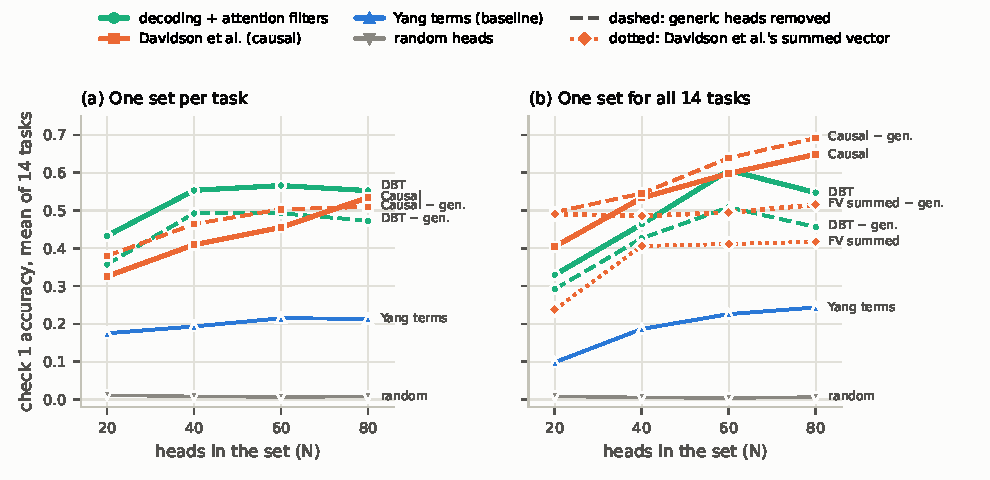
\includegraphics[width=\textwidth]{figures/e13_size}
\caption{Check 1, mean accuracy over the 14 tasks against the number of heads, held-out items, cross-fitted $\alpha\in\{1,2\}$, mean of the two folds. (a) One set per task; (b) one set for all 14 tasks. Solid: the ranking as it is; dashed: the generic heads removed before taking the top $N$; dotted: Davidson et al.'s summed vector (shared only). Random: layer-matched to DBT, five draws. The other filter combinations are in Table~\ref{tab:main}.}
\label{fig:size}
\end{figure}

\begin{table}[tbp]
\centering\small
% Generated by scripts/e13_report.py.
\begin{tabular}{@{}lcccccccccccc@{}}
\toprule
 & \multicolumn{6}{c}{One set per task} & \multicolumn{6}{c}{One set for all 14 tasks} \\
\cmidrule(lr){2-7}\cmidrule(lr){8-13}
Heads (N) & 20 & 40 & 60 & 80 & 100 & 120 & 20 & 40 & 60 & 80 & 100 & 120 \\
\midrule
\multicolumn{13}{@{}l}{\textit{Decoding and attention filters}} \\
\quad D & 0.27 & 0.37 & 0.41 & 0.43 & 0.40 & 0.39 & 0.24 & 0.29 & 0.29 & 0.29 & 0.22 & 0.20 \\
\quad B & 0.13 & 0.22 & 0.23 & 0.23 & 0.22 & 0.23 & 0.11 & 0.25 & 0.41 & 0.40 & 0.44 & 0.45 \\
\quad T & 0.31 & 0.45 & 0.48 & 0.54 & \textbf{0.57} & 0.58 & 0.23 & 0.43 & 0.44 & 0.50 & 0.56 & 0.53 \\
\quad DB & \textbf{0.44} & 0.45 & 0.36 & 0.32 & 0.27 & 0.24 & 0.37 & 0.47 & 0.54 & 0.52 & 0.45 & 0.46 \\
\quad DT & 0.35 & 0.47 & 0.49 & 0.51 & 0.53 & 0.54 & 0.32 & 0.37 & 0.45 & 0.48 & 0.46 & 0.42 \\
\quad BT & 0.42 & 0.54 & \textbf{0.58} & 0.55 & 0.57 & 0.57 & 0.35 & 0.45 & 0.60 & 0.56 & 0.58 & 0.63 \\
\quad DBT & 0.43 & \textbf{0.55} & 0.57 & \textbf{0.55} & 0.48 & 0.41 & 0.33 & 0.46 & 0.61 & 0.55 & 0.51 & 0.53 \\
\quad DBT $-$ generic & 0.36 & 0.49 & 0.49 & 0.47 & 0.37 & 0.34 & 0.29 & 0.43 & 0.51 & 0.46 & 0.47 & 0.46 \\
\midrule
\multicolumn{13}{@{}l}{\textit{Davidson et al.\ (causal score)}} \\
\quad Causal & 0.33 & 0.41 & 0.46 & 0.53 & 0.56 & \textbf{0.61} & 0.40 & 0.53 & 0.60 & 0.65 & 0.68 & \textbf{0.69} \\
\quad Causal $-$ generic & 0.38 & 0.46 & 0.50 & 0.51 & 0.53 & 0.58 & \textbf{0.50} & \textbf{0.55} & \textbf{0.64} & \textbf{0.69} & \textbf{0.71} & 0.69 \\
\quad Davidson FV (summed) & -- & -- & -- & -- & -- & -- & 0.24 & 0.41 & 0.41 & 0.42 & 0.43 & 0.36 \\
\quad Davidson FV $-$ generic (summed) & -- & -- & -- & -- & -- & -- & 0.49 & 0.49 & 0.49 & 0.52 & 0.51 & 0.49 \\
\midrule
\multicolumn{13}{@{}l}{\textit{Baseline}} \\
\quad Yang terms & 0.18 & 0.19 & 0.21 & 0.21 & -- & -- & 0.10 & 0.19 & 0.23 & 0.24 & 0.24 & 0.22 \\
\midrule
\multicolumn{13}{@{}l}{\textit{Control}} \\
\quad Random (DBT layers) & 0.01 & 0.01 & 0.01 & 0.01 & 0.01 & 0.01 & 0.01 & 0.01 & 0.00 & 0.01 & 0.01 & 0.01 \\
\bottomrule
\end{tabular}

\caption{Check 1, mean accuracy over the 14 tasks, held-out items, cross-fitted $\alpha\in\{1,2\}$, mean of the two folds. Bold: the best non-random set in each column. Davidson FV: their summed vector, run on the shared ranking only. Yang terms holds fewer heads than $N$ on some tasks at 60 and 80 (58 and 72 heads on average over tasks and folds). Random: layer-matched to DBT, five draws, at DBT's $\alpha$. Unpatched accuracy: 0.01.}
\label{tab:main}
\end{table}

\begin{itemize}
\item \textbf{Per task, the filters match or beat the causal ranking at every size.} DBT and BT lie above Causal, with or without the generic heads, from 20 to 60 heads and level with it at 80. They reach their level at 40 heads and gain little after, whereas the causal ranking keeps rising with size.
\item \textbf{For one set shared by all tasks, the causal ranking is best.} Shared Causal $-$ generic is the best set at every size and still rising at 80 heads, the highest accuracy of the comparison. Shared DBT and BT reach the shared causal ranking with its generic heads at 60 heads, stay below the one without them, and fall back at 80.
\item \textbf{The two scopes favour different rules.} The causal score does better as one shared ranking than as per-task rankings at every size. DBT and BT do better per task at 20 and 40 heads, and about as well in both scopes at 60 and 80. At 40 heads, the per-task DBT sets are level with Shared Causal $-$ generic.
\item \textbf{The hand-written list stays the weak point.} Yang terms is below every other rule except B alone, at every size and in both scopes, and per task it gains little from more heads.
\item \textbf{Which heads matters, not how many.} Random heads with the same number of heads per layer as DBT do nothing at any size. Control means stay low for every set (Table~\ref{tab:control}), so the gains are task-specific.
\end{itemize}

\subsection{Which filters matter}

\begin{itemize}
\item \textbf{T is the strongest single filter.} Attention to the instruction's task words alone ranks heads better than decoding the task's words (D) or avoiding BOS (B), per task at every size and shared from 40 heads on. Per task, B alone is the weakest filter. D alone carries part of the task, and its shared ranking stops improving at 40 heads.
\item \textbf{B and T together give most of the filters' effect.} BT and DBT are nearly equal in both scopes: D adds nothing once B and T are used. T's task words still come from the lens, so the lens is needed, though not as a filter. DT, without B, is below both. DB is level with BT and DBT or slightly above at 20 heads (shared also at 40), and below them at larger sizes.
\item \textbf{Decoding without T fails at larger sizes.} Per task, DB stays level from 20 to 40 heads and then falls, below D alone at 60 and 80. The loss is mostly on the fact tasks: with the larger DB sets the model describes the query (``Located in the heart of \dots'', ``A UNESCO World Heritage \dots'' on park--country) instead of naming the answer. DBT sets of the same size, which add attention to the task words, give the answer. Shared DB does not fall.
\item \textbf{The filters and the causal score partly agree.} Per task, DBT shares about a third of its heads with Causal of the same size; shared, about half. The median layer of both is about 14; that of the sets that only decode (D, Yang terms) is 16 to 18.
\end{itemize}

\subsection{Generic heads and Davidson et al.'s summed vector}

\begin{itemize}
\item \textbf{Removing the generic heads helps the causal rankings}, in both scopes at nearly every size, most for the shared ranking at 20 heads. That set holds five of the generic heads, and from 40 heads on it holds all of them. Removing them also steadies it across folds: with the generic heads the two folds' Shared Causal-20 differ widely, without them they agree.
\item \textbf{Removing them lowers DBT} at every size and in both scopes. DBT sets hold fewer generic heads (two to five) than the causal sets, and removing these costs accuracy instead of adding it. Whether a generic head harms a set thus depends on the set.
\item \textbf{Davidson et al.'s summed vector is below head-by-head patching of the same heads.} With the generic heads it is below at every size. From 40 heads on, the cross-fit always picks $\alpha=1$, because at $\alpha=2$ the vector fails. At 20 heads it is unstable across folds: at $\alpha=2$ it is the second-best set of fold~1, behind one with four times its heads, and fails in fold~2, so the cross-fitted mean is low. The two folds' top 20 differ by two heads; fold~2's holds the late generic head L31H14. Without the generic heads, the summed vector is level with head-by-head patching at 20 heads but does not improve with more heads, so head-by-head patching overtakes it from 40 on.
\item \textbf{The earlier best set does not hold up.} With the generic heads read on all items, the summed vector without them was the best set found (App.~\ref{app:earlier}). With the generic heads chosen on the choosing half it is no longer ahead: the shared causal sets patched head by head and the per-task filter sets of 40 heads or more lie above it.
\end{itemize}

\subsection{By task type}

The means hide large differences between task types (Table~\ref{tab:groups}; per task in Table~\ref{tab:tasks}).

\begin{table}[tbp]
\centering\small\setlength{\tabcolsep}{3.5pt}
\resizebox{\textwidth}{!}{% Generated by scripts/e13_report.py.
\begin{tabular}{@{}lcccccccccccccc@{}}
\toprule
 & \multicolumn{7}{c}{One set per task} & \multicolumn{7}{c}{One set for all tasks} \\
\cmidrule(lr){2-8}\cmidrule(lr){9-15}
Task type & DBT & DB & T & \begin{tabular}[b]{@{}c@{}}DBT\\$-$gen.\end{tabular} & Causal & \begin{tabular}[b]{@{}c@{}}Causal\\$-$gen.\end{tabular} & Yang & DBT & \begin{tabular}[b]{@{}c@{}}DBT\\$-$gen.\end{tabular} & Causal & \begin{tabular}[b]{@{}c@{}}Causal\\$-$gen.\end{tabular} & \begin{tabular}[b]{@{}c@{}}FV\\sum\end{tabular} & \begin{tabular}[b]{@{}c@{}}FV sum\\$-$gen.\end{tabular} & Yang \\
\midrule
\multicolumn{15}{@{}l}{\textit{20 heads}} \\
\quad Word relations (2) & 0.24 & 0.25 & 0.26 & 0.18 & 0.10 & 0.30 & 0.05 & 0.07 & 0.05 & 0.17 & 0.33 & 0.09 & \textbf{0.42} & 0.00 \\
\quad Morphology (2) & 0.48 & 0.63 & 0.24 & 0.38 & 0.54 & 0.61 & 0.01 & 0.43 & 0.38 & 0.66 & \textbf{0.74} & 0.25 & 0.55 & 0.00 \\
\quad Facts (5) & 0.71 & 0.74 & 0.58 & 0.68 & 0.65 & 0.70 & 0.46 & 0.70 & 0.63 & 0.72 & 0.81 & 0.49 & \textbf{0.87} & 0.27 \\
\quad Sequences (2) & 0.04 & 0.00 & 0.02 & 0.03 & 0.01 & 0.00 & 0.01 & 0.00 & 0.01 & 0.06 & \textbf{0.09} & 0.02 & 0.01 & 0.00 \\
\quad Translations (3) & \textbf{0.33} & 0.22 & 0.13 & 0.14 & 0.00 & 0.00 & 0.00 & 0.03 & 0.01 & 0.09 & 0.19 & 0.05 & 0.18 & 0.00 \\
\addlinespace
\multicolumn{15}{@{}l}{\textit{40 heads}} \\
\quad Word relations (2) & 0.36 & 0.45 & 0.30 & 0.36 & 0.26 & \textbf{0.47} & 0.08 & 0.18 & 0.12 & 0.24 & 0.35 & 0.17 & 0.26 & 0.00 \\
\quad Morphology (2) & 0.64 & 0.70 & 0.27 & 0.56 & 0.65 & 0.78 & 0.01 & 0.53 & 0.57 & 0.73 & \textbf{0.81} & 0.36 & 0.62 & 0.02 \\
\quad Facts (5) & 0.80 & 0.56 & 0.74 & 0.75 & 0.73 & 0.75 & 0.47 & \textbf{0.87} & 0.82 & 0.79 & 0.84 & 0.75 & 0.86 & 0.50 \\
\quad Sequences (2) & \textbf{0.19} & 0.01 & 0.06 & 0.16 & 0.09 & 0.09 & 0.05 & 0.16 & 0.13 & 0.12 & 0.17 & 0.14 & 0.04 & 0.04 \\
\quad Translations (3) & \textbf{0.45} & 0.40 & 0.42 & 0.32 & 0.02 & 0.01 & 0.02 & 0.14 & 0.07 & 0.44 & 0.25 & 0.19 & 0.23 & 0.00 \\
\addlinespace
\multicolumn{15}{@{}l}{\textit{60 heads}} \\
\quad Word relations (2) & 0.40 & 0.42 & 0.40 & 0.38 & 0.35 & \textbf{0.46} & 0.04 & 0.28 & 0.15 & 0.32 & 0.45 & 0.16 & 0.29 & 0.00 \\
\quad Morphology (2) & 0.72 & 0.57 & 0.37 & 0.56 & 0.58 & 0.76 & 0.04 & 0.74 & 0.57 & 0.83 & \textbf{0.88} & 0.34 & 0.58 & 0.00 \\
\quad Facts (5) & 0.82 & 0.39 & 0.79 & 0.76 & 0.78 & 0.79 & 0.51 & \textbf{0.89} & 0.85 & 0.82 & 0.86 & 0.74 & 0.84 & 0.61 \\
\quad Sequences (2) & 0.11 & 0.03 & 0.07 & 0.10 & 0.19 & 0.22 & 0.11 & 0.26 & 0.21 & 0.17 & \textbf{0.29} & 0.16 & 0.00 & 0.04 \\
\quad Translations (3) & 0.46 & 0.32 & 0.38 & 0.33 & 0.08 & 0.07 & 0.01 & 0.49 & 0.34 & \textbf{0.54} & 0.47 & 0.25 & 0.32 & 0.00 \\
\addlinespace
\multicolumn{15}{@{}l}{\textit{80 heads}} \\
\quad Word relations (2) & 0.40 & 0.44 & 0.43 & 0.34 & 0.44 & 0.46 & 0.01 & 0.23 & 0.14 & 0.45 & \textbf{0.55} & 0.17 & 0.34 & 0.00 \\
\quad Morphology (2) & 0.72 & 0.40 & 0.63 & 0.61 & 0.73 & 0.64 & 0.04 & 0.66 & 0.47 & 0.90 & \textbf{0.92} & 0.38 & 0.55 & 0.00 \\
\quad Facts (5) & 0.78 & 0.41 & 0.80 & 0.70 & 0.81 & 0.81 & 0.48 & 0.84 & 0.79 & 0.83 & \textbf{0.86} & 0.72 & 0.84 & 0.66 \\
\quad Sequences (2) & 0.12 & 0.04 & 0.11 & 0.10 & 0.35 & 0.28 & 0.20 & 0.31 & 0.26 & 0.23 & \textbf{0.36} & 0.21 & 0.07 & 0.04 \\
\quad Translations (3) & 0.45 & 0.22 & 0.43 & 0.34 & 0.13 & 0.10 & 0.02 & 0.36 & 0.23 & \textbf{0.58} & 0.58 & 0.23 & 0.36 & 0.00 \\
\addlinespace
\multicolumn{15}{@{}l}{\textit{100 heads}} \\
\quad Word relations (2) & 0.41 & 0.34 & 0.41 & 0.33 & 0.48 & 0.45 & -- & 0.22 & 0.18 & 0.53 & \textbf{0.59} & 0.17 & 0.32 & 0.01 \\
\quad Morphology (2) & 0.60 & 0.33 & 0.64 & 0.46 & 0.83 & 0.71 & -- & 0.58 & 0.48 & \textbf{0.95} & 0.88 & 0.47 & 0.56 & 0.01 \\
\quad Facts (5) & 0.69 & 0.38 & 0.81 & 0.57 & 0.82 & 0.81 & -- & 0.81 & 0.78 & 0.86 & \textbf{0.86} & 0.70 & 0.84 & 0.65 \\
\quad Sequences (2) & 0.07 & 0.04 & 0.12 & 0.05 & 0.38 & 0.31 & -- & 0.25 & 0.25 & 0.20 & \textbf{0.41} & 0.22 & 0.07 & 0.05 \\
\quad Translations (3) & 0.37 & 0.15 & 0.52 & 0.24 & 0.14 & 0.13 & -- & 0.33 & 0.31 & \textbf{0.64} & 0.63 & 0.27 & 0.32 & 0.00 \\
\addlinespace
\multicolumn{15}{@{}l}{\textit{120 heads}} \\
\quad Word relations (2) & 0.38 & 0.24 & 0.42 & 0.31 & \textbf{0.53} & 0.47 & -- & 0.25 & 0.18 & 0.51 & 0.51 & 0.11 & 0.22 & 0.00 \\
\quad Morphology (2) & 0.45 & 0.36 & 0.64 & 0.40 & 0.89 & 0.85 & -- & 0.61 & 0.46 & \textbf{0.95} & 0.83 & 0.40 & 0.57 & 0.01 \\
\quad Facts (5) & 0.61 & 0.33 & 0.83 & 0.50 & 0.82 & 0.81 & -- & 0.79 & 0.75 & \textbf{0.86} & 0.85 & 0.64 & 0.84 & 0.58 \\
\quad Sequences (2) & 0.07 & 0.03 & 0.10 & 0.06 & 0.43 & 0.35 & -- & 0.20 & 0.21 & 0.23 & \textbf{0.44} & 0.11 & 0.06 & 0.04 \\
\quad Translations (3) & 0.31 & 0.14 & 0.58 & 0.23 & 0.26 & 0.21 & -- & 0.43 & 0.32 & \textbf{0.66} & 0.64 & 0.20 & 0.32 & 0.02 \\
\bottomrule
\end{tabular}
}
\caption{Check 1, mean accuracy per task type (number of tasks in brackets) at each set size; held-out items, cross-fitted $\alpha\in\{1,2\}$, mean of the two folds. Bold: highest in the row. BT, close to DBT, is in Table~\ref{tab:main} only.}
\label{tab:groups}
\end{table}

\begin{itemize}
\item \textbf{Facts} (capitals, currency, landmark, park, product) are carried by almost every rule from 20 heads on, shared or not; Yang terms and per-task DB above 40 heads are the exceptions.
\item \textbf{Morphology} is carried best by the causal rankings, most of all the shared one, which from 60 heads gets nearly every item. Per task, DB and DBT also carry it. T alone does little here below 80 heads: present--past has no task word in two of its five templates.
\item \textbf{Translations} are carried by the per-task sets that use attention (BT and DBT at every size), and by no per-task causal ranking at any size. Ranked over all tasks, the causal score does carry them, from 40 heads on, and so do the shared BT and DBT sets from 60. Removing the generic heads lowers the shared causal sets on translations at 40 and 60 heads.
\item \textbf{Sequences} (next-, prev-item) stay low under every rule. They gain most at 60 to 80 heads, with the causal rankings (per task and shared) and Shared DBT.
\item \textbf{Word relations} are carried best by Causal $-$ generic in both scopes from 40 heads on, by the summed vector without generic heads at 20, and per task also by DB.
\end{itemize}

No rule wins every type. Per task, the filters win translations, and the causal ranking without generic heads wins word relations and, up to 60 heads, morphology. No rule carries sequences.

% =====================================================================
\section{Best approaches}\label{sec:best}

For the stated goal, a small set of heads that represents the tasks in general:
\begin{enumerate}
\item \textbf{Read heads with J-head.} It finds more heads that carry the task, in middle layers the logit lens misses, and its lead holds at equal set size.
\item \textbf{One set for all tasks: Shared Causal $-$ generic}, patched head by head. Rank heads by Davidson et al.'s causal score averaged over tasks, drop the generic heads among the top 30, and take the top $N$. It is the best set at every size; 20 heads already carry facts and morphology, and it keeps improving up to 80.
\item \textbf{Without patching, per task: DBT or BT at 40 heads.} Rank heads by attention to the instruction's task words and by low attention to BOS (plus decoding, for DBT). Chosen from J-head readings and attention alone, these sets are close to the best per-task set of any size and level with the shared causal set of the same size.
\item \textbf{Without patching, shared: DBT or BT at 60 heads}, about level with the shared causal ranking with its generic heads at that size.
\item \textbf{Davidson et al.'s summed vector only without its generic heads}, and not beyond 20 heads; the same heads patched one by one do better from 40 heads on.
\item \textbf{By task type}: translations need per-task attention filters, or a shared causal set of at least 40 heads; morphology is carried best by causal rankings; facts by almost any rule from 20 heads; sequences by no set found here.
\item \textbf{Not}: Yang et al.'s hand-written lists, D or B alone, and DB with more than 40 heads per task.
\end{enumerate}

% =====================================================================
\section{Limitations}

One model and 14 simple tasks. Every run is single and greedy, without intervals; rerunning a set with differently made-up batches moves its mean by up to 0.004 (Sec.~\ref{sec:approaches}), so differences of a point or two between sets are not established. Only $\alpha$ 1 and 2 are compared, which may underrate sets that peak higher; sequences peaked at larger $\alpha$ in earlier runs. The generic-head rule was changed during the design. The rule fixed before the per-half runs (heads above the largest drop in the sorted generic score) became unstable once the score was computed on all five templates, where its two largest drops were nearly equal. We replaced it with the two-group split, choosing between the rules on the generic scores alone, not on accuracy. But the split marks the same heads as those per-half runs, whose accuracies we had seen (App.~\ref{app:earlier}). Ranked combination sets at large $N$ hold heads that rank poorly on one filter. T has no task word in three templates (antonym, present--past), so on those tasks it rests on fewer prompts. The word lists keep some word pieces and Japanese fragments. Yang terms has fewer than $N$ heads on seven tasks at 60 and 80 heads. Items are held out, but wordings are not: every set was chosen and tested on the same five templates, so whether the sets carry the task when it is asked differently is untested. The capped comparison runs check~1 only.

\subsection*{Conditions still to run}
The leading sets (Shared Causal $-$ generic, per-task DBT and BT, Shared DBT) on instructions worded differently, to test whether they carry the task when it is asked in other words. The wordings are generated and await a hand check; the run needs new readings.

\paragraph{Code and data.} The capped comparison: word lists \texttt{scripts/e13\_lists.py}, attention pass \texttt{scripts/e13\_attention.py}, sets and generic heads \texttt{scripts/e13\_sets.py}, runs \texttt{scripts/e13\_patch.sh}, which also runs Davidson et al.'s summed vector with \texttt{scripts/e13\_fv\_residual.py}, and tables and figures \texttt{scripts/e13\_report.py}. Results in \texttt{results/e13\_capped}: per fold the word lists, sets, generic heads, accuracies and every patched reply; \texttt{summary.csv} and \texttt{per\_task.csv} at the cross-fitted $\alpha$. The causal scores are those of the first held-out runs (\texttt{results/heldout/fold\{1,2\}/fv}). The reproductions and earlier comparisons: App.~\ref{app:earlier}.

\bibliographystyle{plainnat}
\bibliography{references}

% =====================================================================
\clearpage
\appendix
\section{Per-task results}\label{app:tables}

\begin{table}[H]
\centering\footnotesize\setlength{\tabcolsep}{3pt}
\resizebox{\textwidth}{!}{% Generated by scripts/e13_report.py.
\begin{tabular}{@{}lccccccccccccccc@{}}
\toprule
 &  & \multicolumn{7}{c}{One set per task} & \multicolumn{7}{c}{One set for all tasks} \\
\cmidrule(lr){3-9}\cmidrule(lr){10-16}
Task & Unp. & DBT & DB & T & \begin{tabular}[b]{@{}c@{}}DBT\\$-$gen.\end{tabular} & Causal & \begin{tabular}[b]{@{}c@{}}Causal\\$-$gen.\end{tabular} & Yang & DBT & \begin{tabular}[b]{@{}c@{}}DBT\\$-$gen.\end{tabular} & Causal & \begin{tabular}[b]{@{}c@{}}Causal\\$-$gen.\end{tabular} & \begin{tabular}[b]{@{}c@{}}FV\\sum\end{tabular} & \begin{tabular}[b]{@{}c@{}}FV sum\\$-$gen.\end{tabular} & Yang \\
\midrule
\multicolumn{16}{@{}l}{\textit{Word relations}} \\
antonym & 0.00 & 0.41 & \textbf{0.59} & 0.38 & 0.50 & 0.23 & 0.44 & 0.01 & 0.24 & 0.19 & 0.26 & 0.45 & 0.31 & 0.32 & 0.00 \\
synonym & 0.03 & 0.30 & 0.31 & 0.22 & 0.23 & 0.28 & \textbf{0.51} & 0.16 & 0.12 & 0.06 & 0.22 & 0.25 & 0.04 & 0.20 & 0.01 \\
\multicolumn{16}{@{}l}{\textit{Morphology}} \\
singular--plural & 0.00 & 0.79 & 0.85 & 0.53 & 0.71 & 0.62 & 0.80 & 0.01 & 0.79 & 0.74 & 0.77 & \textbf{0.87} & 0.68 & 0.83 & 0.03 \\
present--past & 0.00 & 0.50 & 0.55 & 0.00 & 0.42 & 0.68 & \textbf{0.76} & 0.00 & 0.27 & 0.41 & 0.69 & 0.76 & 0.04 & 0.41 & 0.00 \\
\multicolumn{16}{@{}l}{\textit{Facts}} \\
country--capital & 0.00 & 0.97 & 0.85 & 0.97 & 0.97 & 0.92 & 0.97 & 0.71 & 0.97 & 0.93 & 0.95 & \textbf{0.98} & 0.64 & 0.96 & 0.63 \\
country--currency & 0.00 & 0.47 & 0.45 & 0.45 & 0.41 & 0.13 & 0.10 & 0.13 & 0.64 & 0.62 & \textbf{0.67} & 0.60 & 0.51 & 0.61 & 0.07 \\
landmark--country & 0.01 & 0.95 & 0.30 & 0.93 & 0.94 & 0.96 & 0.95 & 0.68 & 0.96 & 0.94 & 0.86 & 0.93 & 0.93 & \textbf{0.96} & 0.67 \\
park--country & 0.00 & 0.78 & 0.51 & 0.55 & 0.69 & \textbf{0.89} & 0.84 & 0.47 & 0.88 & 0.79 & 0.68 & 0.82 & 0.86 & 0.89 & 0.49 \\
product--company & 0.07 & 0.84 & 0.70 & 0.81 & 0.76 & 0.77 & \textbf{0.90} & 0.37 & 0.90 & 0.85 & 0.80 & 0.88 & 0.83 & 0.87 & 0.63 \\
\multicolumn{16}{@{}l}{\textit{Sequences}} \\
next-item & 0.00 & 0.10 & 0.01 & 0.05 & 0.06 & 0.15 & 0.04 & 0.02 & 0.14 & 0.10 & 0.10 & 0.10 & \textbf{0.22} & 0.04 & 0.02 \\
prev-item & 0.00 & \textbf{0.28} & 0.01 & 0.07 & 0.27 & 0.03 & 0.14 & 0.08 & 0.18 & 0.16 & 0.14 & 0.23 & 0.07 & 0.03 & 0.06 \\
\multicolumn{16}{@{}l}{\textit{Translations}} \\
English--French & 0.00 & \textbf{0.46} & 0.39 & 0.45 & 0.30 & 0.06 & 0.03 & 0.04 & 0.12 & 0.06 & 0.35 & 0.23 & 0.21 & 0.16 & 0.00 \\
English--German & 0.00 & 0.34 & 0.31 & 0.29 & 0.23 & 0.00 & 0.00 & 0.01 & 0.06 & 0.04 & \textbf{0.37} & 0.19 & 0.08 & 0.14 & 0.00 \\
English--Spanish & 0.00 & 0.55 & 0.51 & 0.54 & 0.43 & 0.01 & 0.01 & 0.01 & 0.24 & 0.10 & \textbf{0.59} & 0.34 & 0.27 & 0.37 & 0.00 \\
\midrule
Mean & 0.01 & 0.55 & 0.45 & 0.45 & 0.49 & 0.41 & 0.46 & 0.19 & 0.46 & 0.43 & 0.53 & 0.55 & 0.41 & 0.49 & 0.19 \\
\bottomrule
\end{tabular}
}
\caption{Check 1 per task at 40 heads, held-out items, cross-fitted $\alpha\in\{1,2\}$, mean of the two folds. Unp.: unpatched accuracy. Bold: the row's highest value.}
\label{tab:tasks}
\end{table}

\begin{table}[H]
\centering\small
% Generated by scripts/e13_report.py.
\begin{tabular}{@{}lcccccccc@{}}
\toprule
 & \multicolumn{4}{c}{One set per task} & \multicolumn{4}{c}{One set for all 14 tasks} \\
\cmidrule(lr){2-5}\cmidrule(lr){6-9}
Heads (N) & 20 & 40 & 60 & 80 & 20 & 40 & 60 & 80 \\
\midrule
\multicolumn{9}{@{}l}{\textit{Decoding and attention filters}} \\
\quad D & 0.03 & 0.02 & 0.02 & 0.02 & 0.01 & 0.01 & 0.01 & 0.02 \\
\quad B & 0.00 & 0.00 & 0.01 & 0.01 & 0.01 & 0.01 & 0.02 & 0.02 \\
\quad T & 0.03 & 0.03 & 0.03 & 0.04 & 0.02 & 0.03 & 0.02 & 0.02 \\
\quad DB & 0.02 & 0.01 & 0.01 & 0.01 & 0.02 & 0.01 & 0.01 & 0.01 \\
\quad DT & 0.04 & 0.03 & 0.02 & 0.01 & 0.02 & 0.01 & 0.01 & 0.01 \\
\quad BT & 0.04 & 0.01 & 0.02 & 0.02 & 0.05 & 0.02 & 0.02 & 0.01 \\
\quad DBT & 0.02 & 0.02 & 0.01 & 0.01 & 0.02 & 0.01 & 0.01 & 0.01 \\
\quad DBT $-$ generic & 0.02 & 0.01 & 0.01 & 0.01 & 0.02 & 0.01 & 0.01 & 0.01 \\
\midrule
\multicolumn{9}{@{}l}{\textit{Davidson et al.\ (causal score)}} \\
\quad Causal & 0.03 & 0.03 & 0.03 & 0.03 & 0.03 & 0.04 & 0.02 & 0.02 \\
\quad Causal $-$ generic & 0.04 & 0.02 & 0.02 & 0.02 & 0.03 & 0.02 & 0.01 & 0.02 \\
\quad Davidson FV (summed) & -- & -- & -- & -- & 0.03 & 0.04 & 0.04 & 0.03 \\
\quad Davidson FV $-$ generic (summed) & -- & -- & -- & -- & 0.03 & 0.03 & 0.04 & 0.05 \\
\midrule
\multicolumn{9}{@{}l}{\textit{Baseline}} \\
\quad Yang terms & 0.03 & 0.03 & 0.02 & 0.01 & 0.04 & 0.05 & 0.02 & 0.01 \\
\midrule
\multicolumn{9}{@{}l}{\textit{Control}} \\
\quad Random (DBT layers) & -- & -- & -- & -- & -- & -- & -- & -- \\
\bottomrule
\end{tabular}

\caption{Control: the sets of Table~\ref{tab:main} patched with the control task's mean (Sec.~\ref{sec:setup}), check~1, mean over the 14 tasks, at the task mean's cross-fitted $\alpha$. Random sets are not run with the control mean.}
\label{tab:control}
\end{table}

% =====================================================================
\section{Task-word lists}\label{app:lists}

The 50 generic words removed from every list, from WikiText-103 (Sec.~\ref{sec:approaches}), by share: % Generated by scripts/e13_report.py.
[Arabic letter], [Devanagari letter], pří, which, mph, http, his, what, https, whilst, pretty, colour, they, their, even, maybe, amongst, programme, only, himself, she, bindingutil, really, again, her, then, also, herself, itself, organisation, sfml, however, behaviors, during, 1, [Thai repetition mark], our, being, ones, [Thai `word'], later, there, him, [Korean `date'], \zh{页面存档备份}, programmes, who, why, local, etc
\unskip. Five of them are not in a Latin, Chinese, Japanese or Cyrillic script and are described in brackets.

\small
% Generated by scripts/e13_report.py.
\begin{xltabular}{\textwidth}{@{}>{\raggedright\arraybackslash}p{1.9cm}>{\raggedright\arraybackslash}p{2.3cm}>{\raggedright\arraybackslash}X>{\raggedright\arraybackslash}p{2.9cm}@{}}
\caption{Task-word lists (fold 1, by share) and the words of each list that occur in the instructions, which T measures attention to. Last column: fold 2's list against fold 1's.}\label{tab:lists} \\
\toprule
Task & T words & 30-word list & Fold 2 \\
\midrule
\endfirsthead
\toprule Task & T words & 30-word list & Fold 2 \\ \midrule
\endhead
antonym & opposite, question, word & opposite, word, instead, because, opposing, words, therefore, definition, reverse, synonyms, whats, name, oppos, meaning, american, ant, answer, synonym, question, likely, adjective, thats, probably, 2, similar, vocabulary, above, either, same, how & $+$english, definitions, 3; $-$above, same, how \\
synonym & synonym, word & synonyms, word, words, 2, similar, synonym, definition, name, whats, english, syn, 3, same, afterward, possibly, instead, called, because, other, american, similarly, therefore, 4, somebody, answer, stuff, how, 5, others, named & $+$definitions; $-$named \\
singular--plural & plural & because, single, name, noun, multiple, plural, lingu, either, linguistic, therefore, names, named, naming, similar, english, called, whats, individual, 2, how, vocabulary, when, same, 3, nouns, identical, sisters, pronunciation, question, very & $+$answer; $-$very \\
present--past & english, verb, word & english, verb, lingu, grammar, name, because, linguistic, question, verbs, gramm, called, word, how, britain, whats, british, 2, language, named, instead, took, sentence, when, either, very, tom, transitioning, did, noun, therefore & $+$england; $-$did \\
country--capital & answer, capital, city, country & city, cities, country, town, countries, answer, international, geography, downtown, capital, canada, american, answers, italy, london, diplomatic, africa, location, città, germany, towns, political, question, named, therefore, usa, very, australia, because, england & $+$france, wikipedia; $-$germany, usa \\
country--currency & answer, country, currency & currency, currencies, country, monetary, money, countries, dollar, international, financial, american, answer, foreign, germany, british, canada, wikipedia, italy, instead, dollars, france, called, nationality, australia, \ja{ンツ}, england, tom, nation, economic, netherlands, \ja{かし} & $+$australian, 2, named, very; $-$england, nation, netherlands, \ja{かし} \\
landmark--country & country, located, where & country, countries, england, canada, germany, france, location, australia, city, international, geography, italy, located, geographical, locations, usa, county, geographic, cities, netherlands, ireland, american, regional, town, named, wikipedia, british, where, nationality, japan & $+$tourism, america; $-$british, nationality \\
park--country & country, located, nation, park & country, countries, england, canada, location, australia, park, located, france, national, tourism, germany, geography, unesco, parks, international, italy, city, nation, tourist, geographical, county, wildlife, locations, british, named, nationality, tourists, american, geographic & $+$usa; $-$tourists \\
product--company & company, product & company, companies, manufacturer, product, microsoft, manufacturers, products, because, named, name, owned, wikipedia, software, apple, ownership, respectively, answer, manufacturing, mitsubishi, ibm, how, \ja{ーダ}, question, very, probably, windows, 2, japanese, nintendo, production & $+$computer; $-$japanese \\
next-item & after, item, next, sequence & next, january, july, september, november, october, february, sequence, because, question, items, december, june, after, item, april, 2, calendar, answer, christmas, seven, when, 3, math, eight, monday, six, nine, each, named & $+$sunday, friday, tuesday, wednesday, saturday, thursday, 4, answers; $-$february, june, april, seven, eight, six, each, named \\
prev-item & before, item, previous, return, sequence & previous, preceding, prior, answer, question, item, next, because, items, sequence, january, previously, earlier, september, answers, how, november, october, before, preced, questions, july, 2, return, february, seven, when, therefore, whats, december & $+$monday, sunday, 3, christmas; $-$february, seven, therefore, whats \\
English--French & english, french, translation; fold 2: english, french, into, translation & french, france, english, paris, \zh{法国}, translation, italian, european, american, \ru{француз}, translations, language, linguistic, japanese, german, françois, called, bilingual, therefore, languages, how, named, name, quebec, translated, foreign, portuguese, lingu, franc, 2 & $+$into, behaviour; $-$foreign, 2 \\
English--German & english, german, translation & german, germany, germans, english, european, berlin, french, american, translation, linguistic, language, deutschland, called, therefore, italian, von, japanese, munich, czech, translations, languages, lingu, die, bav, austria, bilingual, named, name, auf, austrian & $+$british; $-$austrian \\
English--Spanish & english, spanish, translation & spanish, english, mexican, hispanic, translation, bilingual, spain, language, mexico, translations, portuguese, linguistic, french, ilingual, called, languages, american, name, maría, madrid, santiago, therefore, japanese, because, lingu, italian, méxico, named, translated, synonyms & none \\
\bottomrule
\end{xltabular}

\normalsize

% =====================================================================
\section{Earlier selection rules}\label{app:earlier}

Before the capped comparison, the rules were compared at the sizes each produced: per-task sets of every head passing a threshold, a few fixed sizes (20 and 40 heads), and shared rankings at 5 to 40 heads (Table~\ref{tab:earlier}, Figure~\ref{fig:earlier}). These runs led to the present design and are kept for reference. They differ from it in four ways. The word lists were each task's most active decoded words under an English-frequency filter, with no generic words removed. T's task words were Yang et al.'s terms and the task's 10 most task-specific decoded words. The generic heads were the six read on all items, so the sets without them were not cleanly held out. Both checks were run.

\paragraph{Names.} \emph{Yang terms}: heads that decode a term of Yang et al.'s list on $\geq$10\% of the best template's prompts. \emph{Task+common}: heads that decode one of the task's 5 most task-specific and 5 most common decoded words on $\geq$10\% of prompts; \emph{Task+common-$N$} its top $N$ by that rate; \emph{instr.\ diff.}\ the same rule on the clean-minus-corrupted instruction readings. \emph{Causal-$N$} and \emph{Causal-matched} (as many heads as Task+common): Davidson et al.'s ranking per task. D, B, T and their combinations: every head passing the named thresholds (D: decodes a list word on $\geq$10\% of prompts; B: BOS attention $\leq$0.5; T: task-word attention $\geq$0.05); D$_{10}$, DB$_{10}$ with a 10-word list. \emph{Shared causal-$N$}, \emph{Shared DBT-30}: shared rankings. \emph{Davidson FV-30}: their summed vector with the 30 heads chosen over the 14 tasks. \emph{Random, X layers}: as many heads per layer as X, outside it; \emph{Random from D, X size}: X's size drawn from D.

\begin{table}[tbp]
\centering\small
% Generated by scripts/synthesis_report.py.
\begin{tabular}{@{}lccccc@{}}
\toprule
Head set & Heads & \multicolumn{2}{c}{Check 1} & \multicolumn{2}{c}{Check 2} \\
\cmidrule(lr){3-4}\cmidrule(lr){5-6}
 & median (range) & task & control & task & control \\
\midrule
\multicolumn{6}{@{}l}{\textit{One set per task}} \\
\quad Decoded words (lens) & & & & & \\
\qquad Yang terms & 26 (8--48) & 0.17 & 0.03 & 0.27 & 0.09 \\
\qquad Task+common-20 & 20 & 0.16 & 0.03 & 0.27 & 0.10 \\
\qquad Task+common-40 & 40 & 0.22 & 0.05 & 0.31 & 0.10 \\
\qquad Task+common & 118 (98--146) & 0.40 & 0.05 & 0.34 & 0.13 \\
\qquad Task+common, instr.\ diff. & 107 (84--128) & 0.18 & 0.01 & 0.33 & 0.10 \\
\quad Causal score (Davidson et al.) & & & & & \\
\qquad Causal-20 & 20 & 0.33 & 0.03 & 0.34 & 0.10 \\
\qquad Causal-40 & 40 & 0.41 & 0.03 & 0.39 & 0.12 \\
\qquad Causal-matched & 118 (98--146) & 0.59 & 0.04 & 0.39 & 0.12 \\
\quad Filters: decoding (D), not BOS (B), task-word attention (T) & & & & & \\
\qquad D$_{10}$ & 110 (80--134) & 0.34 & 0.04 & 0.32 & 0.10 \\
\qquad DB$_{10}$ & 32 (18--42) & 0.31 & 0.02 & 0.34 & 0.13 \\
\qquad D & 249 (210--274) & 0.41 & 0.02 & 0.26 & 0.05 \\
\qquad DB & 65 (52--84) & 0.51 & 0.01 & 0.32 & 0.09 \\
\qquad DBT & 38 (3--47) & 0.49 & 0.03 & 0.35 & 0.14 \\
\qquad BT & 94 (12--114) & 0.45 & 0.02 & 0.38 & 0.13 \\
\qquad T & 154 (13--302) & 0.55 & 0.02 & 0.40 & 0.11 \\
\quad Random heads & & & & & \\
\qquad Random, Task+common-20 layers & 20 & 0.01 & -- & 0.08 & -- \\
\qquad Random, Task+common-40 layers & 40 & 0.01 & -- & 0.10 & -- \\
\qquad Random, Task+common layers & 118 (98--146) & 0.02 & -- & 0.12 & -- \\
\qquad Random from D$_{10}$, DB$_{10}$ size & 32 (18--42) & 0.07 & -- & -- & -- \\
\qquad Random from D, DB size & 65 (52--84) & 0.13 & -- & 0.18 & -- \\
\qquad Random, DB layers & 65 (52--84) & 0.01 & -- & 0.08 & -- \\
\qquad Random from D, DBT size & 38 (3--47) & 0.06 & -- & 0.14 & -- \\
\qquad Random, DBT layers & 38 (3--47) & 0.01 & -- & 0.08 & -- \\
\qquad Random, T layers & 154 (13--302) & 0.18 & -- & 0.16 & -- \\
\midrule
\multicolumn{6}{@{}l}{\textit{One set for all 14 tasks}} \\
\quad Causal score (Davidson et al.) & & & & & \\
\qquad Davidson FV-30 ($\alpha{=}1$) & 30 & 0.39 & 0.05 & 0.34 & 0.16 \\
\qquad Davidson FV-30 $-$ generic & 25 & 0.63 & 0.05 & 0.41 & 0.13 \\
\qquad Shared causal-20 & 20 & 0.40 & 0.03 & 0.34 & 0.12 \\
\qquad Shared causal-40 & 40 & 0.53 & 0.04 & 0.38 & 0.14 \\
\qquad Shared causal-20 $-$ generic & 18 & 0.51 & 0.04 & 0.39 & 0.14 \\
\quad Filters: decoding (D), not BOS (B), task-word attention (T) & & & & & \\
\qquad Shared DBT-30 & 30 & 0.47 & 0.01 & 0.38 & 0.10 \\
\qquad Shared BT-30 & 30 & 0.44 & 0.02 & 0.38 & 0.15 \\
\qquad Shared DB-30 & 30 & 0.43 & 0.02 & 0.36 & 0.18 \\
\quad Random heads & & & & & \\
\qquad Random shared, causal-20 layers & 20 & 0.01 & -- & 0.06 & -- \\
\qquad Random shared, DBT-30 layers & 30 & 0.01 & -- & 0.06 & -- \\
\bottomrule
\end{tabular}

\caption{Earlier rules: mean accuracy over the 14 tasks, held-out items, cross-fitted $\alpha\in\{1,2\}$, mean of the two folds. Heads: median (range) over tasks. Davidson FV-30: their intervention at their $\alpha=1$. Unpatched accuracy: 0.01 (check 1), 0 (check 2). The generic heads of the $-$ generic rows were read on all items. Removing the generic heads of Sec.~\ref{sec:approaches} instead, chosen on each half, lowers Davidson FV-30 $-$ generic from 0.63 to 0.49 and Shared causal-20 $-$ generic from 0.51 to 0.42 in check~1.}
\label{tab:earlier}
\end{table}

\begin{figure}[tbp]
\centering
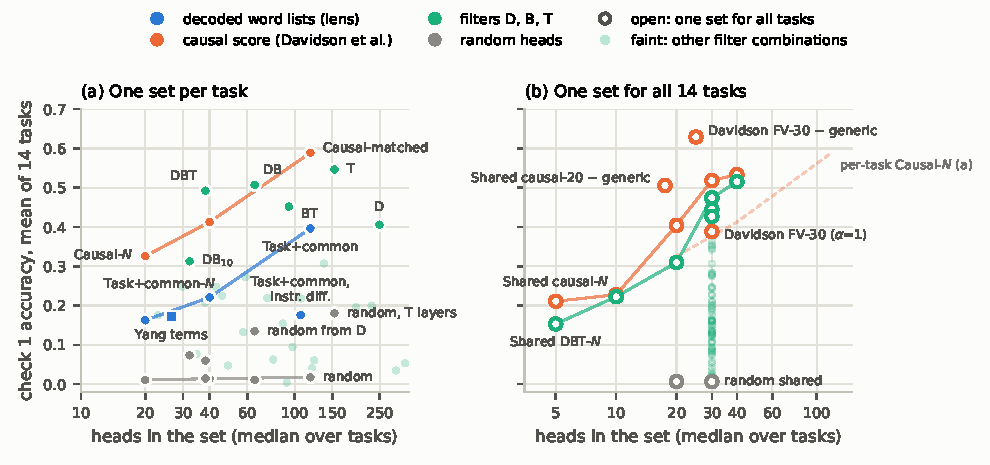
\includegraphics[width=\textwidth]{figures/synth_size}
\caption{Earlier rules, check 1 against the number of heads (median over tasks; log scale). (a) One set per task; (b) one set for all tasks. Colour: how heads are scored; filled: per task; open: shared; square: Yang terms. Lines join one ranking at increasing size. Faint dots: the other filter combinations.}
\label{fig:earlier}
\end{figure}

What these runs showed, and what the capped comparison was built to test:
\begin{itemize}
\item Random heads with the same layers did nothing; random decoders did little; control means stayed low in check~1.
\item The hand-written list was the weak point of the lexical method: decoded-word lists more than doubled its mean, but only at about 120 heads.
\item At the sizes run, a causal ranking beat decoded words at every fixed size, and Causal-matched (about 120 heads) had the highest per-task mean.
\item Attention filters closed most of that gap without patching: DB and DBT (40--65 heads) lay above Causal-40, and T (about 150 heads) close to Causal-matched. Attention to the query or to the rest of the instruction lowered every combination.
\item Task types rested on different heads: causal rankings carried morphology and sequences, the attention filters translations and word relations, and facts were carried by almost any good set.
\item Check~2 (1-shot prompts answered wrongly) did not separate good sets from mediocre ones: random sets reached a quarter of the best, and every non-random set lay between 0.26 and 0.41.
\item Sets of different sizes could not be compared directly, and the best shared result depended on generic heads read on all items. Both led to the capped comparison.
\end{itemize}

Some single tasks rest on very few heads (Table~\ref{tab:small}; chosen and scored on the same items, so optimistic).

\begin{table}[H]
\centering\small
\begin{tabularx}{\textwidth}{@{}llLc@{}}
\toprule
Task & Heads & How chosen & Check 1 \\
\midrule
country--capital & L16H25 alone & attends to \emph{capital}, \emph{country} in the instruction and decodes \emph{city} & 0.88 \\
landmark--country & 5 & top 5 by attention to task words $\times$ decoding & 0.79 \\
product--company & 20 & same rule, top 20 & 0.72 \\
singular--plural & 20 & same rule, top 20 & 0.68 \\
present--past & L15H1 alone & found in the top-5 J-head set; example-style means only (check 2: 0.76) & 0.80 \\
landmark / product & 5--10 & Davidson et al.'s FV with fewer heads, $\alpha$ 3--4 & 0.95 / 0.87 \\
\bottomrule
\end{tabularx}
\caption{Small sets that carry one task (exploratory: chosen and scored on the same items, best $\alpha$ on them). Controls are low except product--company with the 5--10-head FV (0.22).}
\label{tab:small}
\end{table}

Other rules that did not help: heads passing Yang et al.'s rule under all five templates (better only on facts); word lists without a contrast between tasks; the weakest task's score for shared sets; head scores from GPT-5.5 reading each head's top tokens (two tasks: matched Task+common-20 on country--capital, nothing below 60 heads on English--German).

\paragraph{Code and data.} Tables and figures of this appendix and of Sec.~\ref{sec:repro}: \texttt{scripts/synthesis\_report.py}, from the saved result files. Folders under \texttt{results/}: Yang terms, Task+common, Task+common-$N$, Causal-$N$, Causal-matched and their layer-matched random sets in \texttt{heldout} (report \texttt{paper/e4\_heldout}); Task+common, instr.\ diff.\ in \texttt{diff\_heads}; D$_{10}$, DB$_{10}$ in \texttt{e7\_attfilter} (\texttt{paper/e7-attention-filter}); D, DB, DBT, BT, T in \texttt{e8\_filters} (\texttt{paper/e8-filter-combos}); Shared DBT-30, DB-30, BT-30 in \texttt{e10\_shared}; Shared causal-$N$, Shared DBT-$N$ at the other sizes, Davidson FV-30 with and without generic heads, and the other random sets in \texttt{e11\_complete}; the per-half generic heads in \texttt{e12\_generic\_halves}.

\end{document}
